% !TeX root = ../../main.tex
\section{Probabilità Condizionata}

La probabilità condizionata di un evento $A$ rispetto a un evento $B$ è la probabilità che si verifichi $A$, sapendo che l'evento $B$ è già accaduto.
\\Questa probabilità, indicata con $\mathbb{P}(A \mid B)$ (oppure $\mathbb{P}_B(A)$), esprime una ``correzione'' o un aggiornamento delle aspettative su $A$ dettato dall'osservazione di $B$.

La definizione formale è data dalla formula:
\[
\mathbb{P}(A \mid B) = \frac{\mathbb{P}(A \cap B)}{\mathbb{P}(B)}
\]
dove:
\begin{itemize}
    \item $\mathbb{P}(A \cap B)$ è la \textbf{probabilità congiunta} (l'intersezione), ovvero la probabilità che i due eventi si verifichino entrambi;
    \item $\mathbb{P}(B)$ è la \textbf{probabilità dell'evento condizionante} (che deve essere diversa da zero).
\end{itemize}

Inoltre vale la seguente relazione:
\[
\mathbb{P}(B \mid A) = \frac{\mathbb{P}(A \cap B)}{\mathbb{P}(A)} \iff \mathbb{P}(A \cap B) = \mathbb{P}(B \mid A)\mathbb{P}(A) = \mathbb{P}(A \mid B)\mathbb{P}(B)
\]

Questa relazione prende anche il nome di legge della probabilità composta.

\begin{esempio}[Esempio con il dado]

Consideriamo il lancio di un dado a 6 facce non truccato ($\Omega = \{1, 2, 3, 4, 5, 6\}$). Definiamo i seguenti due eventi:
\begin{itemize}
    \item \textbf{Evento A:} esce un numero dispari
    \[ A = \{1, 3, 5\} \]
    \item \textbf{Evento B:} esce un numero compreso tra 3 e 5
    \[ B = \{3, 4, 5\} \]
\end{itemize}

Ci chiediamo: \emph{qual è la probabilità che si verifichi $A$ sapendo che $B$ è già avvenuto?}
\\Possiamo risolvere il problema in due modi:

\subsubsection*{1. Applicando la formula matematica}

Calcoliamo le singole probabilità basandoci sullo spazio campionario totale del dado:
\begin{itemize}
    \item L'intersezione $A \cap B$ contiene gli elementi comuni ai due insiemi: $\{3, 5\}$.
    \\Quindi $\mathbb{P}(A \cap B) = \frac{2}{6}$.
    \item La probabilità di $B$ è data dai suoi 3 elementi su 6 totali: $\mathbb{P}(B) = \frac{3}{6}$.
\end{itemize}

Applicando la formula:
\[
\mathbb{P}(A \mid B) = \frac{2/6}{3/6} = \frac{2}{3}
\]

\subsubsection*{2. Interpretazione insiemistica (Approccio intuitivo)}

Possiamo ragionare in modo più diretto pensando al concetto di \textbf{restrizione dello spazio campionario}.
\\Poiché sappiamo che $B$ si è verificato, il nostro ``nuovo universo'' non è più l'intero dado (6 facce), ma solo l'insieme $B$ ($\{3, 4, 5\}$).
\\La domanda diventa quindi: \emph{``Quanti elementi di $A$ sono contenuti dentro $B$?''}

\begin{itemize}
    \item L'insieme $B$ ha 3 elementi totali (casi possibili).
    \item Tra questi, gli elementi che appartengono anche ad $A$ (dispari) sono il 3 e il 5, quindi sono 2 (casi favorevoli).
\end{itemize}

Di conseguenza, la probabilità è 2 su 3, ovvero:
\[
\frac{2}{3}
\]

\end{esempio}

\begin{esempio}[Probabilità Condizionata (Studenti di Algebra eChimica)]

\textbf{Traccia del problema:}
In una certa scuola ci sono 500 studenti. 
\begin{itemize}
    \item 150 studenti sono iscritti al corso di Algebra ($A$).
    \item 80 studenti sono iscritti al corso di Chimica ($C$).
    \item 30 studenti frequentano entrambi i corsi ($A \cap C$).
\end{itemize}
Se viene scelto uno studente a caso:
\begin{enumerate}
    \item[(a)] Qual è la probabilità che lo studente frequenti Algebra?
    \item[(b)] Qual è la probabilità che lo studente frequenti Chimica sapendo che frequenta anche Algebra?
    \item[(c)] Qual è la probabilità che lo studente frequenti Algebra sapendo che frequenta anche Chimica?
\end{enumerate}

\begin{center}
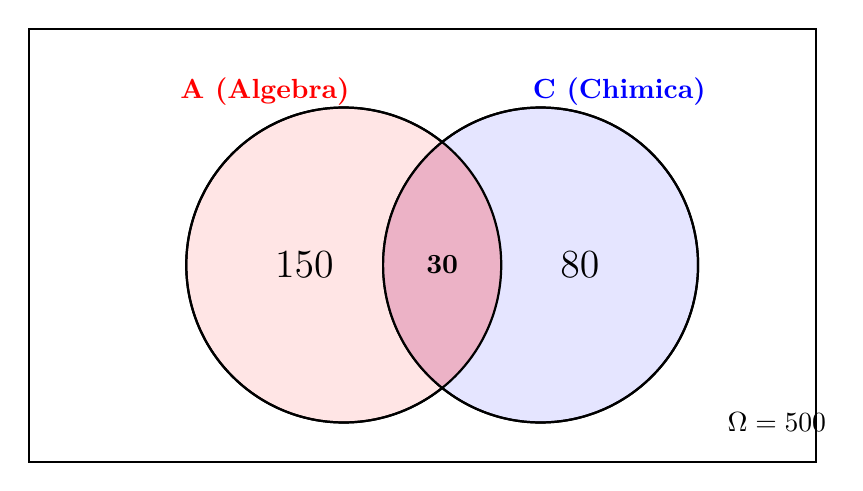
\begin{tikzpicture}
    % Rettangolo Universo
    \draw[thick] (-4,-2.5) rectangle (6,3);
    \node at (5.5,-2) {$\Omega = 500$};
    
    % Cerchio A (Algebra)
    \draw[thick, fill=red!10] (0,0) circle (2cm);
    \node[red, font=\bfseries] at (-1, 2.2) {A (Algebra)};
    
    % Cerchio C (Chimica)
    \draw[thick, fill=blue!10] (2.5,0) circle (2cm);
    \node[blue, font=\bfseries] at (3.5, 2.2) {C (Chimica)};
    
    % Intersezione
    \begin{scope}
        \clip (0,0) circle (2cm);
        \fill[purple!30] (2.5,0) circle (2cm);
    \end{scope}
    \draw[thick] (0,0) circle (2cm); % Ridisegna contorno A
    \draw[thick] (2.5,0) circle (2cm); % Ridisegna contorno C
    
    % Etichette Numeriche
    % Solo Algebra: 150 tot - 30 inters = 120
    \node[font=\Large] at (-0.5,0) {150}; 
    
    % Intersezione
    \node[font=\Large, font=\bfseries] at (1.25,0) {30};
    
    % Solo Chimica: 80 tot - 30 inters = 50
    \node[font=\Large] at (3,0) {80};
    
\end{tikzpicture}
\end{center}

\subsubsection*{Soluzione}

\paragraph{(a) Probabilità semplice: $\mathbb{P}(A)$}
La domanda è: \emph{Qual è la probabilità che uno studente scelto a caso studi Algebra?}
\\Qui lo spazio campionario è l'intera scuola ($\Omega$). Non abbiamo informazioni aggiuntive, quindi usiamo il totale degli studenti come denominatore.

\[
\mathbb{P}(A) = \frac{\text{Studenti di Algebra}}{\text{Totale studenti}} = \frac{150}{500} = \frac{3}{10} = 30\%
\]

\paragraph{(b) Probabilità condizionata: $\mathbb{P}(C \mid A)$}
La domanda è: \emph{Sapendo che lo studente studia Algebra, qual è la probabilità che studi anche Chimica?}
\\L'informazione ``studia Algebra'' riduce il nostro universo (\textbf{restrizione dello spazio campionario}). Ignoriamo i 500 totali; ora contano solo i 150 studenti di Algebra.
\\Tra questi 150, quelli che fanno anche Chimica (l'intersezione) sono 30.
\\Domandiamoci: Quanti studenti che studiano chimica studiano anche algebra?

\[
\mathbb{P}(C \mid A) = \frac{\text{Studenti (Algebra e Chimica)}}{\text{Studenti di Algebra}} = \frac{30}{150} = \frac{1}{5} = 20\%
\]
\emph{Nota: L'informazione ha corretto l'aspettativa base di Chimica (che sarebbe $80/500 = 16\%$) portandola al $20\%$.}

\paragraph{(c) Probabilità condizionata inversa: $\mathbb{P}(A \mid C)$}
La domanda è: \emph{Sapendo che lo studente studia Chimica, qual è la probabilità che studi anche Algebra?}
\\Ora la condizione restringe l'universo ai soli 80 studenti di Chimica.
\\Tra questi 80, quelli che fanno anche Algebra sono sempre gli stessi 30 (l'intersezione è commutativa).

\[
\mathbb{P}(A \mid C) = \frac{\text{Studenti (Algebra e Chimica)}}{\text{Studenti di Chimica}} = \frac{30}{80} = \frac{3}{8} = 37,5\%
\]
\emph{Nota: L'informazione ha corretto l'aspettativa base di Algebra dal $30\%$ al $37,5\%$.}

\paragraph{Conclusione}
In entrambi i casi condizionati (b) e (c), il numeratore rimane lo stesso (l'intersezione $30$), ma il denominatore cambia in base all'evento che sappiamo essere già accaduto, modificando così la probabilità finale.

\end{esempio}

